\chapter{Employee Turnover Forecasting for Human Resource Management Based on Time Series Analysis}\label{ch:timesereis}
\section{Introduction}
Employee turnover has drawn researchers' and human resource managers' attention because organizations lack  niche skill sets and resources, which require time and planning to acquire at crucial times. The hiring lead time is often long, particularly when special skills are involved. In some organizations, like U.S. national laboratories, the process can take months because of security-clearance requirements. Therefore, a good employee-turnover prediction at the firm and departmental levels is essential for effective human resource planning (HRP), budgeting, and recruiting. 

Human resource planning is an ongoing systematic planning process to optimize the human resource pool. For organizations to efficiently and effectively execute tasks, the right people must be available at the right places at the right time \citep{khoong1996}. Over the years, organizations have scaled up their efforts in manufacturing, marketing and financing. However, organizations have always struggled to develop sustainable HRP models  \citep{heneman1993}, whose objective is to match employees and jobs to avoid manpower shortages or surpluses \citep{cambal2011}. To achieve this balance, employee turnover is often central to organizational workforce planning and strategy.

As summarized in Table \ref{tab:1}, researches developed employee turnover models using various statistical methods. Previous studies have identified employee-turnover explanatory predictors. For instance, \citet{bluedorn1982} related turnover to the individual's, routine, age, service length, and perception of environmental opportunities. \citet{balfour1993} suggested that caseworkers with more education, less experience, and less stake in an organization are more likely to turnover. \citet{wright1998} associated emotional exhaustion with job performance and subsequent turnover, but not with job satisfaction. Predicting employee turnover based on employee absenteeism and performance, \citet{morrow1999} pstudy showed a positively correlated absenteeism and voluntary turnover as well as negatively correlated performance ratings and voluntary turnover. \citet{thaden2010} indicated that organizational culture may potentially be an important factor for retaining workers.   
\begin{landscape}% Landscape page
\pagestyle{empty}%	
	\begin{table}[htbp]
		\centering
		\scriptsize
		\caption{Summary of Previous Research on Employment Turnover Forecast}
		\begin{tabular}{L{2.8cm}  L{2.8cm}  C{1.2cm}  L{3cm} C{1.2cm}  C{1.5cm} C{1.5cm} C{1.5cm}  L{2.8cm}}
			\toprule
			Authors (Year) & Data Acquisition &  Data Horizon & Methods & Software & Economic Indicator & Response Variable & Estimate & Model Evaluation \\
			\midrule
			Bluedorn (1982)& Employee records and Survey & 1 year & Correlations, multiple regression & N/A & No & Number & Point with intervals& $R^2=0.22$, Adjusted $R^2=0.11$ \\
			
			Ng et al. (1991) & Survey & N/A   & Hazard proportional model & BMDP 2L & No    &  Probability  & Point with intervals & Pair t-test  \\
			
			Balfour et al. (1993) & Employee records  & 33 months & Non-linear logistic regression & N/A   & No    & Probability  & Point & Chi-square values  \\
			
			Feeley et al. (1997) & Survey & 60 months & Social network, logistic regression, correlation & NEGOPY, UCINET & No    & Probability  & Point & $R^2=0.23$ \\
			
			Wright et al. (1998) & Survey & 1 year & Hypothesis test, correlation, logistic regression  & N/A   & No    & N/A   & N/A   & Correlation r=0.34, $P<0.01$ \\
			
			Morrow et al. (1999) & Demographic information and employee records & 2 years & Logistic regression, correlation & N/A   & No    & Probability  & Point & (-2 log likelihood) chi-square=193.13 \\
			
			Sexton et al. (2005) & Demographic information and employee records & 10 years (yearly) & NN    & FORTRAN  & Yes   & Leave or not & Point & Type I error=0.25\% Type II error=5.83\% \\
			
			Hong et al. (2007) & Survey & N/A   & Logit and probit model & SPSS  & No    & Probability  & N/A   & $R^2=0.5$, Quadratic Probability Scores = 0.18 for training and 0.12 for test \\
			
			Nagadevara et al. (2008) & Demographic information and employee records & 3 years & NN, logistic regression, classification/regression trees, discriminant analysis & N/A   & No    & Leave or not & Point & Contingency table \\
			
			Thaden et al. (2010) & Survey & 2 years & Multiple regression & N/A   & No    & Duration & Point with intervals &  $R^2=0.56$, $P< 0.001$ \\
			
			Größler and Zock (2010) & Employee records & 360 months & System dynamics  & N/A   & No    & Number & Point & N/A \\
			
			Saradhi et al. (2011) & Survey & 2 years & SVMs, random forest,  Naïve Bayes classifiers & N/A   & No    & Probability  & Point & True/false positive rate and precision \\
			
			Alao et al. (2013) &  Employee records   & 28 years (yearly) & Decision tree & WEKA See5 & No    & Probability  & Point & True/false positive rate and precision \\
			Tews et al. (2014) & Employee records and Survey & 6 months & Logistic regression & N/A   & No    & Probability & Point & $R^2=0.23$ \\
			Collini et al. (2015) & Survey and turnover rates   & 1 year & Correlation and Regression & N/A   & No    & Turnover rates & Point & No \\
			
			\bottomrule
		\end{tabular}%
		\label{tab:1}%
	\end{table}%
\end{landscape}
Other insights have been gained from more recent research. For instance, according to \citet{tews2014}, personal events, professional events, internal work events and constituent attachment are highly related to turnover. \citet{collini2015} found that interpersonal respect, mission fulfilment, and engagement are statistically significant predictors for turnover in health care. However, these researchers found that diversity climate is not related to turnover. Finally, only \citet{sexton2005} considered outside economic variables, unemployment index, and consumer price index in the employee-turnover forecasting model. However, their final model did not include these variables.  
\citet{ferrara2014} in the {\it International Journal of Forecasting} revealed new interest in forecasting business cycles with some complex methodologies. However, forecasting business-cycle turning points is quite difficult, and \citet{hamilton2011} suggested that "the best econometricians can do is probably to nowcast recessions; that is, to recognize a turning point as soon as it occurs, or soon thereafter." An outside variable might facilitate this situation.

Meanwhile, other studies have tried to build turnover prediction models through such techniques as regression, neural network (NN), and data mining. For example, \citet{ng1991} used a proportional hazards regression (PHR) to develop a turnover-prediction model.In \citet{sexton2005}'s study, NN combined with a modified genetic algorithm was used to build a turnover-prediction model. \citet{alao2013} applied a decision tree to the employees' demographical information and personnel records to identify attributes contributing to employee turnover. In these studies, the data source was acquired from either human resource employment records and demographical information or surveys with time horizons ranging from 1 to 28 years. Most of the data was monthly, which is ideal for time series forecasting models.

Although some efforts have been made to predict employee-turnover behaviour, no study has investigated the prediction of employee turnover with time series forecasting techniques. Therefore, this study attempted to fill this research gap. The advantages of a time series forecasting approach are that identifying turnover's determinants is unnecessary and evaluating either a planned or unplanned intervention's effects is helpful  \citep{velicer2003}.  

This chapter  has four parts. The introduction covers the paper's objective and a literature review. Part two identifies tools used in finding time series patterns and in preparing the data for analysis as well as specific forecasting methods. Part three provides the study's results. Part four includes the study's practical implications and limitations.   
\section{Methods}
\subsection{Data Preparation}
 A large multipurpose research organization in the U.S. provided the human resource data. The dataset consisted of over 8,000 observations of active and terminated employees' with incomplete demographic information (including metrics such as payroll category, hired date, termination date, age, years of service, gender, job classification, and department code) from November 2000 to January 2012. The turnover dataset was summarized in the form of monthly data in which each field represented the number of employees leaving the organization. For this research, turnover is defined as the total  number of employees leaving the organization each month. This definition is used as a unit of measurement for the turnover prediction. 

This study examined several economic indicators: unemployment rate index, New York Stock Exchange, U.S gasoline price, and U.S monthly composite leading indicator (CLI). However, only the CLI that the Organization for Economic Co-operation and Development (OECD) published from November 2000 to January 2012 significantly improved the forecasting performance as a predictor of employee turnover's cyclical component because in practice,  the CLI is an early indication of turning points in the macro-economic cycle. OECD constructed the CLI data by aggregating seven components: the number of dwellings started, net new orders for durable goods, share prices-NYSE composite, consumer-sentiment indicator, average weekly hours manufacturing workers worked, purchasing manager index, and spread of interest rates \citep{oecd2013}. The index construction's weights is not released by OECD.
\subsubsection{Pattern Analysis, Cross-correlations, and Outlier Identification}
 To model a time series, looking for patterns in the turnover series is important. First, it is simply applied with a time plot of the series and box plots of the seasons or months. In this case, the turnover series' seasonal pattern were tested using Kruskal-Wallis and ANOVA tests  ($P<0.05$), which did not correct for any trend in the series. The second stage of the pattern analysis involves autocorrelation (ACF) and partial autocorrelation (PACF) plots to identify seasonal, autoregressive, and moving average patterns. If external variables exist (as in this case), the third stage of pattern analysis examines the cross-correlations between turnover series ($Y_t$) and external variables (CLI ($X_t$) over time). The cross-correlation function (CCF) is used to identify lags of CLI($X_t$) ), which might be useful predictors of the turnover series ($Y_t$).  A longer lag that is strong enables the forecast horizon to be longer when using an external variable.

All of the previous stages of the pattern analysis can be contaminated by outliers, so identifying outliers before fitting the actual forecasting model is important. Box plot analysis by seasons can be used to informally flag outliers; however, this approach tends to over-identify outliers. In contrast, ARIMA methods in conjunction with statistical process control (SPC) tend to correctly identify the number of outliers in a series. Conservative ARIMA models ((1,0,1) or (0,1,1)) are used in this control charting. First, the residuals from ARIMA (1,0,1) are divided by the root mean square error to standardize them, and then the outliers are identified with the value greater than $\pm3$ standard deviations from zero by the standardized residuals' scatterplots  \citep{alwan1988, grznar1997}.
Identifying the outliers using SPC and then smoothing them is a way to both refine the data for further analysis and facilitate finding the underlying pattern in the data series. Smoothing outliers in a time series is essential  to eliminate  random noise and other irregularities. When the outlier is identified, it is adjusted to be more similar to its neighboring points \citep{grznar1997}. In this study, unusual observations were smoothed using a nonlinear data smoothing method, based on repeated medians (RMD) of a five-period span (as shown in equation \ref{eq:1}) \citep{velleman1980},
%equation1
\begin{equation} \label{eq:1}
	S_t=Median(y_{t-2s},y_{t-s},y_t,y_{t+s},y_{t+2s} ) 
\end{equation}
where $S_t$ is the actual smoothed value at time t, $y_t$ is value of response variable at time $t$, and $s$ is the number of total seasonal periods, which is 12. This smoothing is only performed on potential outliers within their season and not across adjacent periods. Sometimes outliers can distort normality, white noise, cross correlations, ACF and PACF, and the model's predictive performance. Thus, properly dealing with outliers means asking hard questions about these unusual observations from a human resource perspective; in turn, answering those questions can add understanding and improved forecasting ability.    The outliers are not always unusual events but interventions or change points needing  to be accommodated in the model.  In this kind of human-resource dataset, such abnormalities could be the following: retirement incentives were offered, another company was purchased, a section of the original company was sold, or the potential outlier might reflect an economic down turn.  Many possibilities of abnormalities exist; but if outliers are not over identified, a good human resource department should be able to provide quick answers in unusual s ituations.
\subsection{Time Series Analysis}
In time series forecasting, past observations of the variable are collected and analysed to develop a model describing the pattern. This modelling approach is particularly useful when little knowledge is available regarding  the data-generating process or when no satisfactory explanatory model relates the prediction variable to other explanatory variables \citep{zhang2003}. In this study, univariate and multivariate time series methods were used to identify an optimum forecast. Number Cruncher Statistical System (NCSS), SAS, and R were the statistical software used. Two data partitions were analysed: the training sample (November 2000–January 2011) and the holdout sample (February 2011—January 2012). For each model, the training sample was used to build the model while the holdout sample was used to validate the model because the most recent time series data is considered the most important factor for prediction purposes \citep{bergmeir2012}. 
\subsection{Univariate Methods (without External Variables)}
Univariate time series analysis models without external variables use months for seasonality and trend as turnover predictors. The univariate models used in this study were time series regression, decomposition, Winter's Exponential Smoothing (WES), and Box-Jenkins Autoregressive Integrated Moving Averages (ARIMA). One critical reason for selecting these models was to avoid restricting the forecasting horizon, i.e., how far in the future predictions could be made. 

\subsubsection{Time Series Regression}
The univariate time series regression model used trend and seasonality as predictors. The additive time series regression model with intercept, trend, monthly seasonality, and error terms took the form shown in Equation \ref{equation:reg},
\begin{equation}
	\label{equation:reg}
	Y_t = \beta_0+\beta_1 x_{trend} + \sum_{i=2}^{12} {\beta_i d_i}+\xi_i
\end{equation}
where, $Y_t$ is response variable at time $t$,  $\beta_i$ is the coefficients estimated by regression, $x_{trend}$ is a continuous variable representing trend with value from 1 to $n$, $d_i$ is dummy variable representing seasonal periods. In addition, the additive regression models with interventions (pulse or steps) were also analyzed because of because of the downsize policy in certain time points, which are denoted by dummy variable in the regression function. The multiplicative time series regression model with intercept, trend, monthly seasonality, and error terms was also considered with the form as shown in Equation \ref{eq:mulreg},
\begin{equation}
	\label{eq:mulreg}
	Ln(Y_t)=\beta_0+\beta_1 x_{trend} +\sum_{i=2}^{12} {\beta_i d_i}+\xi_i                              
\end{equation}
where, $Ln(Y_t)$ is natural log transformation of $Y_t$. For these regression models, the significance of the model and the variables were examined by using p-value at 0.05 significance level, lack of collinearity, good holdout performance, and valid regression assumptions. 
\subsubsection{Decomposition}
Decomposition time series methods attempt to separate the series into four components: trend, cycle, seasonality, and irregularity. Multiplicative decomposition methods are expressed globally in Equation \ref{eq:decom}.  
\begin{equation}
	\label{eq:decom}
	Y_t  =f(trend,cycle,seasonality,irregularity)=T_t  C_t S_t I_t            
\end{equation}
The decomposition model can be used assuming no cyclical variation exists, or the cyclical variation can be extracted and fit to  a model to enhance forecasting. Decomposition models can be quite complex, but the classical multiplicative decomposition model in NCSS was used for this turnover series as an easier application.

\subsubsection{Winters Exponential Smoothing (WES)}
WES models work well on series that have either seasonality or both seasonality and trend.  The models can also be additive or multiplicative+, but the preferred option tends to have an additive trend and either additive or multiplicative seasonality.  The multiplicative trend in these kinds of time series models tends to over or under forecast future values. Although dampened models can help avoid this future forecast problem, care must be taken because the forecasts will have a short horizon \citep{de1998}. The robustness and accuracy of Winter's exponential smoothing methods have led to their widespread use in applications where a large number of series necessitates an automated procedure \citep{win1960,tay2003}. WES model is easy to interpret and easily understood by management or those less technically inclined. 
\subsubsection{Autoregressive Integrated Moving Average (ARIMA)}
Statisticians George Box and Gwilym Jenkins introduced the ARIMA models \citep{box1970}, whose general form is ARIMA (p,d,q) where p, d, and q are non-negative integers that refer to the order of the model's autoregressive, integrated, and moving average parts,  respectively. In addition, ARIMA models can handle seasonality, in which case their forms are ARIMA (p,d,q)(P,D,Q). Thus, a series' seasonal factor could have autoregressive, differencing, or moving average patterns.  Because they provide a wide class of models for univariate time series forecasting, ARIMA methods are popular with some forecasters \citep{har1983}.  

\subsection{Univariate Methods (with External Variables)}
Univariate models incorporating an external variable (CLI) as a predictor of a turnover series' cyclical component were also examined. It included dynamic regression and more complex decomposition models.
\subsubsection{Dynamic Regression with External Variable}
The dynamic regression model describes how the forecasting output is linearly related to current and past values of one or more input series. Two assumptions are critical for the dynamic regression model. First, the input series' observations occur at equally spaced time intervals. Second, the output does not affect the input series \citep{pankratz2012}. Dynamic regression models allow inclusion of   external variables, interventions, and transfer functions. In this study, the external variables (CLI and interventions) were incorporated into the dynamic regression model. Equation \ref{eq:reg2} is a simple representation of the model with trend, seasonal dummy variable, and interventions:
\begin{equation}
Y_t = \beta_0+\beta_1 x_{trend} + \sum_{i=2}^{12} {\beta_i d_i}+\varpi_0 I_t +\frac{\varpi_1}{1-\delta_1 B} I^{'}_t +\xi_i
\label{eq:reg2}
\end{equation}
where $I_t$ is a dummy variable representing pulse and step periods, and $I^{'}_t$ is a dummy variable representing pulse periods. Also, $\varpi_0$, $\varpi_1$, and $\theta_1$ are the change-point coefficients that regression estimates and $1-\delta_1 B$ refers to the delayed rise or fall in the forecast variable.
  
\subsubsection{Decomposition with External Variable}
In this more complex decomposition model, CLI and its lag terms predict   a cyclical component in the decomposition model. This research applied two approaches to obtain a decomposition model: the automatic decomposition in NCSS with the cyclical variable (CLI) incorporated, and a multiplicative decomposition model built with the product of the best ARIMA and cyclical factor (CLI). 
\subsection{Nonlinear and Multivariate Methods}
\subsubsection{State Space Model}
A state space model consists of an observation equation as shown in equation \ref{eq:ssm1} and a Markovian transition equation as shown in Equation \ref{eq:ssm2} 
\begin{equation}
y_t=F_t \theta_t +v_t
\label{eq:ssm1}
\end{equation}
\begin{equation}
\theta_t=G_t\theta_{t-1} + w_t
\label{eq:ssm2}
\end{equation}
where $y_t$ is a $m \times 1$ data vector; $\theta_t$  is a $p\times1$ unknown state-vector, $F_t$ is a $m\times p$ state vector relating the observation data to the state vector $\theta_t$, and $G_t$ is a $p\times p$ state transition matrix. In addition, $v_t$, $w_t$ are random error matrices which independently and identically follow a multinomial distribution. State space models were modelled using R {\tt stats}, {\tt dlm}, and {\tt forecast} packages. 

\subsubsection{Vector Autoregressive Model}
Vector autoregressive model (VAR) is an econometric model for multivariate time series analysis. It is an extension of the univariate autoregressive model,i.e., each variable is represented as a linear function of its lags and the other variables' lags. VAR models are often used to describe and forecast financial and economic time series. A VAR model consists of a set of k variables (also called endogenous variables) $y_t=〖(y_{1t}, y_{2t}, \dots, y_{kt})$, denoted as $k\times1$ vector. A $p^{th}$ order VAR model is expressed as 
\begin{equation}
y_t=c+A_1y_{t-1}+\dots +A_py_{t-p}+e_t
\end{equation}
where $A_i(k \times k)$ is a coefficient matrix. Also, $e_t$  is a $k \times 1$ unobservable white noise vector process where expected value of this vector is zero and a time-invariant covariance matrix $E(e_t e_t^{'})=\sum$. The R {\tt vars} package models the VAR model.
\subsection{Model Evaluation}
A good forecasting model should be evaluated in term of predictive ability, goodness of fit using the $R^2$, mean absolute percentage error (MAPE), mean absolute error (MAE) or other fit diagnostics, normality tests on residuals, and a white noise test on those same residuals to ensure that no time series pattern is left. The best fitting model is generally selected based on a higher $R^2$ value in the holdout data, a lower MAPE, normally distributed residuals, and passing a white noise test. 

To evaluate the time series methods, the pseudo $R^2$ for training and holdout data were calculated as standard criteria to test the goodness of model fitting as expressed in Equation \ref{eq:rsquare}.
\begin{equation}
	\label{eq:rsquare}
	R_{pseudo}^2=1-\frac{\sum_{t=1}^{n}(y_t-\hat{y_t})}{\sum_{t=1}^{n}(y_t-\bar{y_t})}
\end{equation}

MAPE was another measure of the time series model fitting methods' accuracy as shown in equation \ref{eq:mape} \citep{Hanke1998, Bowerman2005}. This measure was used to compare the model performance for the specific dataset by using time series methods since it measured relative performance \citep{Chu1998} as reflected in Equation \ref{eq:mape}.
\begin{equation}
	\label{eq:mape}
	MAPE=\frac{\sum_{t=1}^{n}\left | \frac{y_t-\hat{y_t}}{y_t} \right |}{n}
\end{equation}

A good time series model should have normally distributed residuals. In this study, the residuals' normality was evaluated using two powerful normality tests: Shapiro-Wilk \citep{Shapiro1965} and D'Agostino Omnibus normality test \citep{d1990} in NCSS.

The white noise test is performed on the residuals to check for any undetected time series pattern still remaining in the residuals and not accounted for by the model. Independent residuals, those residuals' random scatter, or no time series pattern in residuals  \citep{Weisent2010} is always preferred when choosing a best model. In practice, the Q-statistic (also called the Box-Pierce statistic or the Ljung-Box statistic) is used as an objective diagnostic measure of white noise for a time series to compare whether the autocorrelations from residuals and white noise are statistically significantly different. This test statistic is illustrated in Equation \ref{eq:white}:
\begin{equation}
	\label{eq:white}
	Q=n(n+2)\sum_{i=1}^k{\frac{ACF(i)^2}{n-i}}
\end{equation}
where $k$ is selected from the lesser of two seasonal cycles, one-fourth of the observations, or 24 when two seasonal cycles are much greater than 24. In most cases, if a model is lacks white noise, this model is deficient and has to be rectified \citep{de1998}. 
%%%%%%%%%%%%%%%%%%%%%%%%%%%%%%%%%%%%%%%%%%%%%%%
%%%%%%%%%%%%%%     Time Series Result and discussion   %%%%%%%%%%%%%%%%%
%%%%%%%%%%%%%%%%%%%%%%%%%%%%%%%%%%%%%%%%%%%%%%%
\section{Results and Discussion}
\subsection{Employ Turnover Patterns and Outlier Identification}
The time-based turnover series was restructured so that it could be analysed both to observe patterns like trend or seasonality and to understand any inherent time series in the data for further investigation in that direction. 
As shown in Figure \ref{fig:1} (a) the series contains a clear seasonality pattern. The box plot for the turnover series from the ANOVA test confirms this seasonality pattern. In addition, there is a decreasing trend from January to November as shown in Figure \ref{fig:1} (b); then the trend line rises in December. The points labeled  2008 in Figure \ref{fig:1} (b) are considered outliers since they are beyond the upper whiskers. After all the ARIMA models were tested, three outliers appeared in the SPC chart (as shown in Figure \ref{fig:2}); the box plot analysis also flagged two of these outliers. 
\begin{figure}
	\centering
	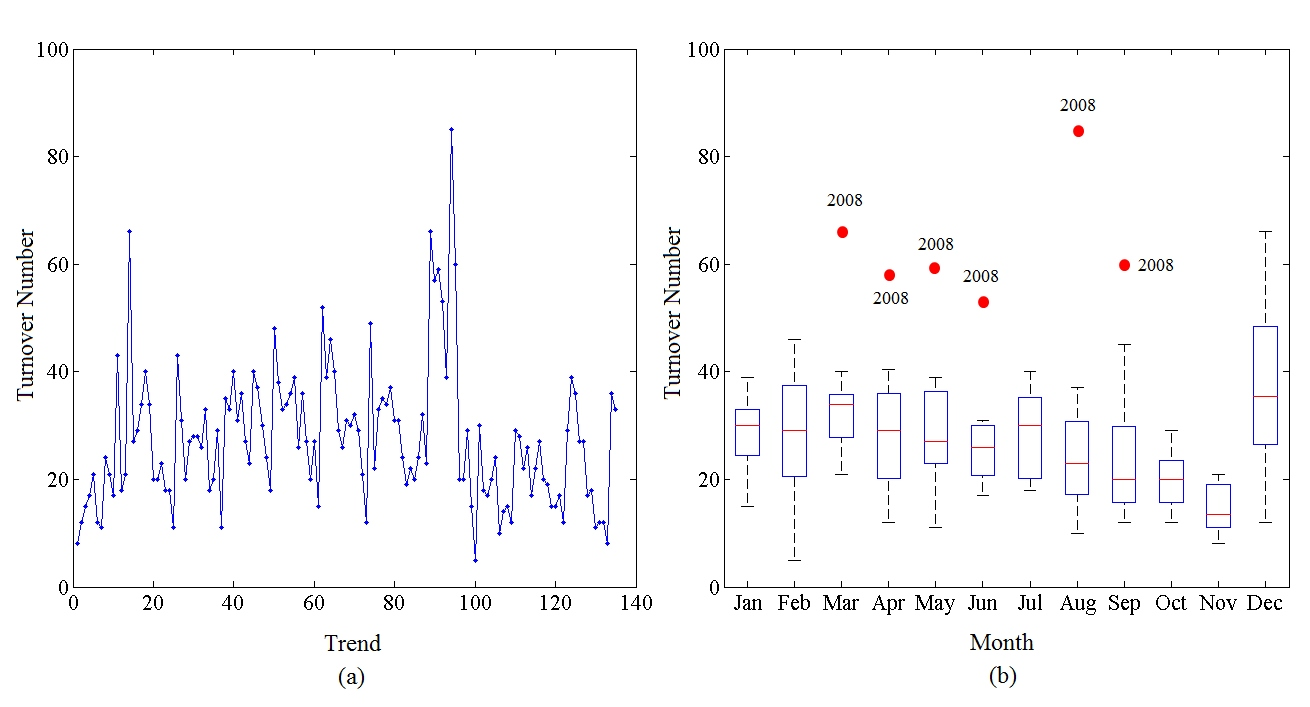
\includegraphics[width=5in]{Fig1.jpg}
	\caption{(a) Monthly Turnover Series Plotted over Time and (b) Box Plot of Turnover Data.}
	\label{fig:1}
\end{figure}
\begin{figure}
	\centering
	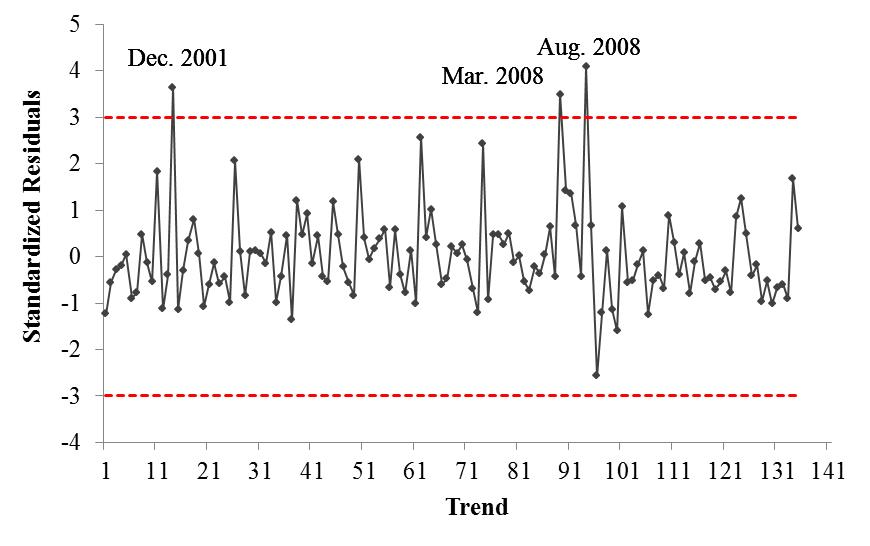
\includegraphics[width=5in]{Fig2.jpg}
	\caption{SPC Chart for Standardized Residuals.}
	\label{fig:2}
\end{figure}Combining the outliers identified by ANOVA test and SPC, 7 outliers were identified. Those outliers are December 2001, March 2008, April 2008, May 2008, June 2008, August 2008, and September 2008. While December 2001 and March 2008 to July 2008 were treated as temporary pulse and steps, August 2008 was treated as pulse with gradual decay in the dynamic regression with intervention methods. In other methods, these outliers were smoothed to soften their impacts, which were univariate regression without intervention, decomposition, exponential smoothing, ARIMA, state space, and vector autoregressive methods. Whenever outliers exist, the cause must be investigated. For instance, December 2001 represents a 9/11 lag impact on job hiring with stronger background checking and increased retiring/hiring. The outliers in 2008 reflect the downsize policy issued in January 2008 with a three months' response-time window to accommodate the organization's voluntary reduction in workforce. 

The ACF and PACF plots for the turnover series are shown in Figure \ref{fig:3} (a, b). The pattern of unsmoothed data in the ACF and PACF hints at ARIMA(1,0,1) with some type of seasonality, but the seasonal pattern is not obvious.
\subsection{Cross-correlations}
The cross-correlation was applied between the turnover series and the CLI series to identify significant lag correlations. The cross-correlations between first differences  for turnover and the CLI series were examined \citep{de1998}, and a “pre-whitening” process for the two series was used to identify cross-correlation patterns \citep{box1970, bowie1981}.
% Department of Sciences at Pennsylvania State University, 2014).
Based on all these calculations, CCFs from Lag 0 to Lag 8 were found to be statistically significant, indicating that the turnover series has a statistically significant correlation with CLI and its 8 lags.  When using the cyclical variable for forecasting, the CLI and its 8 lags were incorporated into the dynamic regression, decomposition, and ARIMA model, respectively.  
\begin{figure}
	\centering
	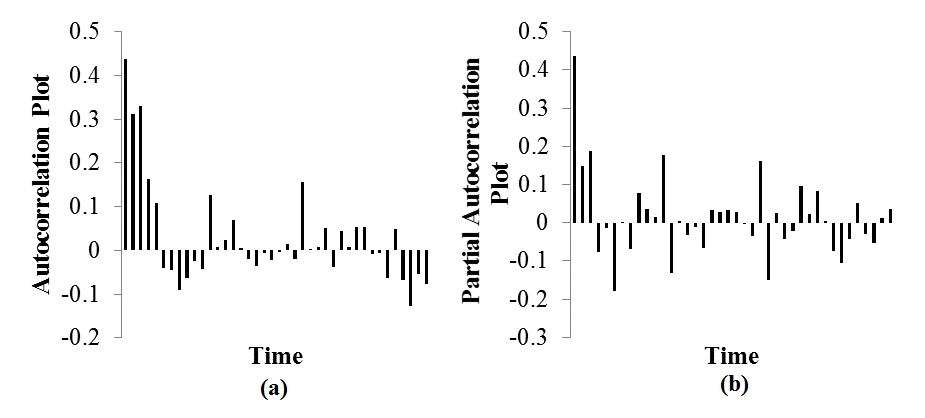
\includegraphics[width=5.5in]{Fig3.jpg}
	\caption{(a) Autocorrelation and (b) Partial autocorrelation plots.}
	\label{fig:3}
\end{figure}


\subsection{Forecasting Results and Comparisons}
Forecasting evaluations for the time series models are provided in the Appendix: Table \ref{tab:allmodels}, Table \ref{tab:dynamic}, Table \ref{tab:arima}, and Table \ref{tab:decomp}. Based on the evaluation statistics, eight univariate models were selected because of an acceptable $R^2$ value for training and holdout data as well as their residual statistics that are optimum among the other models' statistics (as shown in Table \ref{tab:1}). On average, the holdout $R^2$ value of these eight models is 0.51 (ranging from 0.40 to 0.59). 
% Table generated by Excel2LaTeX from sheet 'Sheet1'
\begin{table}[htbp]
	\small %table fond
	\centering
	\caption{Statistics for Selected Time Series Models}
	\smallskip
	\begin{threeparttable}
		\begin{tabular}{C{2cm}p{0.5cm}m{5cm}C{0.8cm}C{1.5cm}ccc}%p: top m: middle
			\hline
			\multicolumn{1}{c}{Method} & \#    & \multicolumn{1}{c}{Model} & Pred $R^2$\tnote{1} & Holdout $R^2$& \multicolumn{1}{c}{MAPE}  & \multicolumn{1}{c}{Normality\tnote{2}} & \multicolumn{1}{c}{WN\tnote{3}} \\
			\hline
			\multirow{5}{2cm}{Univariate without external variable } & U1    & Regression with additive trend and seasonality & 0.51  & 0.57  & 26.15 & No    & No \\
			& U2    & Regression with additive trend, seasonality and intervention4  & 0.72  & 0.52  & 22.84 & Yes   & No \\
			& U3    & Decomposition & 0.65  & 0.54  & 17.97 & Yes   & Yes \\
			& U4    & WES with additive trend and seasonality & 0.52  & 0.52  & 20.65 & Yes   & Yes \\
			& U5    & ARIMA(1,0,1)(0,1,1) & 0.47  & 0.4   & 22.89 & Yes   & Yes \\  \hline
			\multirow{3}{2cm}{Univariate with external variable} & V1    & Dynamic regression using  lag7 CLI as predictor\tnote{4} & 0.77  & 0.59  & 19.91 & Yes   & Yes \\
			& V2    & Decomposition using  lag1 CLI as cycle & 0.65  & 0.55  & 17.97 & Yes   & Yes \\
			& V3    & ARIMA combining with lag1 CLI as cycle & 0.37  & 0.41  & 22.73 & Yes   & Yes \\
			\hline
		\end{tabular}%
		\begin{tablenotes}
			\item[1] Pred. $R^2$ is predicted $R^2$ value for training data.
			\item[2] Normality is residuals' normality test.
			\item[3] WN is white noise test
			\item[4] The data is unsmoothed (or outliers are unadjusted) so as to take advantage of time series models that can accommodate interventions.
		\end{tablenotes}
	\end{threeparttable}
	\label{tab:1}%
\end{table}%

\subsubsection{Univariate Methods (without External Variables)}
The regression model with additive trend and seasonality has the highest holdout $R^2$ (0.57) among the univariate models without external variables, indicating the model's ability to explain 57\% of the holdout sample's total variation. This model is statistically significant ($P<0.05$) for the model and parameters. However, the residuals are not normally distributed and the model does not pass the white noise test. 

The regression model with additive trend, seasonality, and interventions (pulse and step) performs well with a training  $R^2$ of 0.72 and a holdout $R^2$ of 0.52, indicating the model's ability to explain 72\% of the training data's total variation and 52\% of the holdout sample's total variation. This model is statistically significant ($P<0.05$) for the model and parameters. The model has normally distributed residuals, but does not have white noises. However, this regression model captures the spike in December 2001 and sharp fluctuations from March 2008 to August 2008 as shown in Figure \ref{fig:4}. 
\begin{figure}
	\centering
	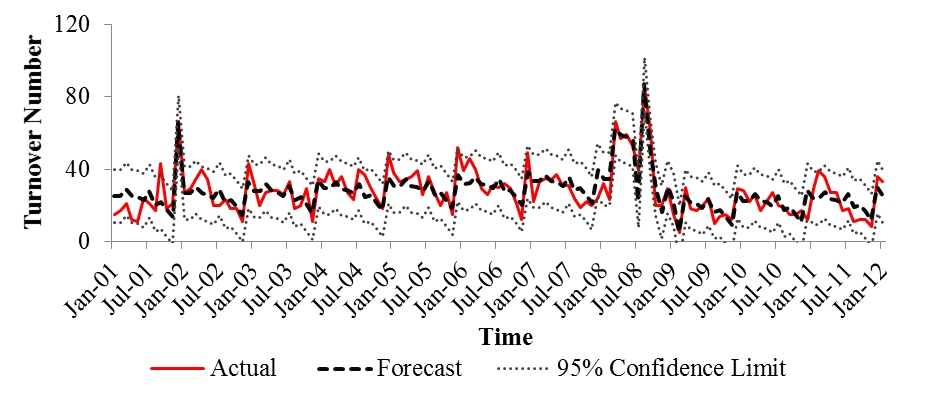
\includegraphics[width=5.5in]{Fig4.jpg}
	\caption{Regression with Interventions Forecast vs. Actual Turnover Number Plot.}
	\label{fig:4}
\end{figure}
The decomposition model was considered as the best univariate model without external variables because this model has a reasonably high training $R^2$ value (0.65), a good holdout $R^2$ value (0.54), and a low MAPE (17.97). This model's residuals are normally distributed and have a white noise pattern. Figure \ref{fig:5} plots the predicted turnover based on the decomposition model and the actual turnover number for the holdout dataset. This plot validates the decomposition model's holdout performance as it mimics the changes in trend and the turnover's seasonality. Furthermore, the prediction is close to the actual turnover numbers. However, this model seems to over-forecast for the six months  June through November.
\begin{figure}
	\centering
	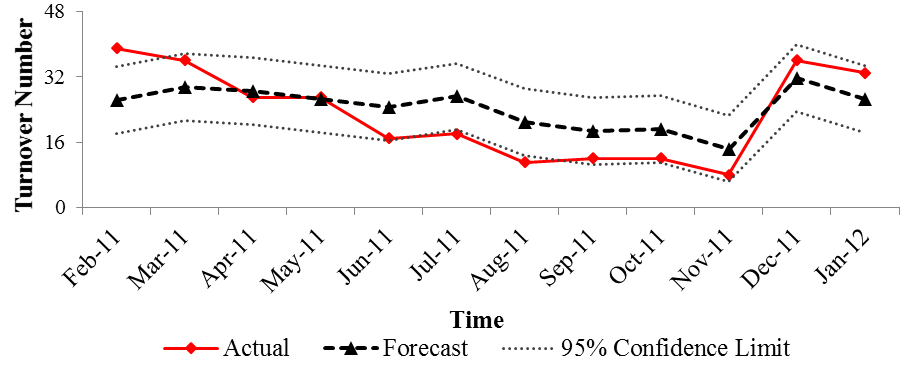
\includegraphics[width=5.5in]{Fig5.png}
	\caption{Decomposition Validation Forecast vs. Actual Turnover Number with Prediction.}
	\label{fig:5}
\end{figure}

\subsubsection{Univariate Methods (with External Variables)}
According to the cross-correlation analysis result, CLI and its 8 lags were applied in dynamic regression, decomposition model, and ARIMA(1,0,1)(0,1,1) respectively as external variable to forecast turnover number. The dynamic regression model with additive trend, seasonality, interventions (pulse and step), and lag7 of CLI is the best model, because it has highest predicted and holdout $R^2$ value (0.77 and 0.59), normal residuals, and white noise. The dynamic regression is globally statistically significant and individually significant for the parameters ($P<0.05$).
\begin{figure}
	\centering
	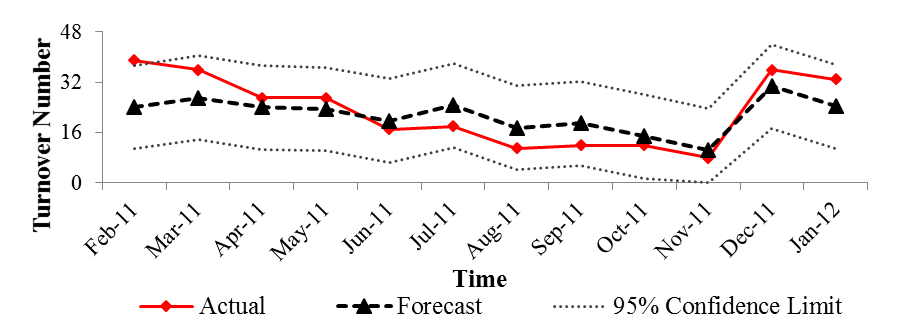
\includegraphics[width=5.5in]{Fig6.png}
	\caption{Dynamic Regression with Lag7 CLI Forecast vs. Actual Turnover Number for Holdout Dataset.}
	\label{fig:6}
\end{figure}
Figure \ref{fig:6} shows the predicted and actual turnover number plots for holdout dataset from the dynamic regression model. Although there was under forecasting from July to September as well, the differences between forecasting values and actual values were much smaller. Compared with top-rated univariate methods without external variables, the dynamic regression model's performance was much improved after using CLI as an outside cyclical variable. 

\subsubsection{Nonlinear and Multivariate Methods (with External Variables)}
State space models with various combinations of errors, trend, seasonality, or an exogenous variable (CLI here) and VAR models of bivariate time series (turnover and CLI) were employed to forecast turnover number (as shown in Table \ref{tab:2}). The exponential smoothing state space model with multiplicative error, no trend, and multiplicative seasonality had the highest holdout $R^2$ value (0.43) among all state space models, which the $R^2$ forecast package automatically selected from 27 exponential smoothing state space models. The residuals have white noise and are normally distributed. However, the training and holdout $R^2$ value (0.53 and 0.43) are relatively lower than the univariate regression models . 
 
Table \ref{tab:2} shows that the VAR models perform better than state space models. The VAR (4, constant, trend, and seasonality) was considered as the best among all these nonlinear and multivariate model with the highest training and holdout $R^2$ values (0.62 and 0.64, respectively). The residuals are normally distributed and have white noise. However, variables in this model (lag terms of turnover and CLI) are not statistically significant, indicating the model is over fitted. Only VAR (1, constant, trend, and seasonality) has significant lag 1 term  of both turnover and CLI. This model also has higher training and holdout $R^2$ values (0.57 and 0.47, respectively) and white noise. However, its residuals are not normally distributed. 
 
The bivariate time series (turnover and CLI) does not have a multivariate moving average pattern, ; thus, it is not  statistically significant. Therefore, the vector moving average (VMA) and vector autoregressive moving average (VARMA) methods were not used to forecast. The volatility models (Garch (1,1) and stochastic volatility model) and nonlinear models (nonlinear autoregressive model and nonlinear threshold autoregressive model) were also considered. However, all these models have lower training and holdout $R^2$ values and higher MAPE values. Therefore, these models' statistics are not provided in the Table \ref{tab:2} due to their poor performance.
\begin{table}[]
	\centering
	\caption{Statistics for Selected Nonlinear and Multivariate Models}
	\scriptsize
	\begin{threeparttable}
	\begin{tabular}{L{1.5cm}cL{3.5cm}ccccc}
		\toprule
		\multicolumn{1}{c}{Method} & \#    & \multicolumn{1}{c}{Model} & Pred. $R^2$ & Holdout $R^2$ & MAPE  & Normality & WN \\
		\midrule
		\multirow{6}[2]{*}{State Space} & S1    & Trend, Seasonality & 0.27  & 0.39  & 24.8  & No    & Yes \\
		& S2    & Trend, Slope, Seasonality & 0.23  & 0.32  & 28.58 & Yes   & Yes \\
		& S3    & Trend, Slope, Seasonality, CLI as regressor & 0.13  & 0.32  & 28.89 & Yes   & Yes \\
		& S4    & Exponential Smoothing (M,N,M) \tnote{1} & 0.51  & 0.43  & 21.14 & Yes   & Yes \\
		& S5    & Structural TS (Level, Slope)  & 0.46  & -0.16 & 22.82 & No    & No \\
		& S6    & Structural TS (Level, Slope, Seasonality)  & 0.51  & 0.04  & 21.47 & Yes   & Yes \\ \midrule
		\multirow{7}[2]{1.2cm}{Vector Autoregressive \tnote{2} } & VA1   & VAR(5, Constant, Seasonality) & 0.62  & 0.49  & 18.2  & No    & Yes \\
		& VA2   & VAR(5, Trend, Seasonality) & 0.63  & 0.52  & 18.37 & Yes   & Yes \\
		& VA3   & VAR(1, Constant, Trend, Seasonality) & 0.52  & 0.47  & 21.08 & No    & Yes \\
		& VA4   & VAR(2, Constant, Trend, Seasonality) & 0.59  & 0.44  & 19.63 & Yes   & Yes \\
		& VA5   & VAR(3, Constant, Trend, Seasonality) & 0.61  & 0.51  & 19.06 & Yes   & Yes \\
		& VA6   & VAR(4, Constant, Trend, Seasonality) & 0.62  & 0.64  & 18.44 & Yes   & Yes \\
		& VA7   & VAR(5, Constant, Trend, Seasonality) & 0.65  & 0.61  & 17.98 & Yes   & Yes \\
		\bottomrule
	\end{tabular}%
	\begin{tablenotes}
   \item[1]	M, N, M is multiplicative errors, no trend, multiplicative seasonality, respectively. 
   \item[2]	VAR(p) is pth order of  lag term. 
	\end{tablenotes}
	\end{threeparttable}
	\label{tab:2}%
\end{table}%

Even more non-linear and multivariate models were considered, but the intent of this research was not to search for a best model but to find a simplistic one  that human resource management (HRM) could use. Noteworthy is that a combination model might have been better than the dynamic regression model, but this study was trying to keep the model  as simple as possible for HRM.
%%%%%%%%%%%%%%%%%%%%%%%%%%%%%%%%%%%%%%%
%%%%%    Time series analysis Conclusion  %%%%%%%%%%%%%%%%%%%
%%%%%%%%%%%%%%%%%%%%%%%%%%%%%%%%%%%%%%%
\section{Conclusion}
In this study, various time series forecasting models for predicting employee turnover were tested and optimal models for turnover forecasts were identified. As a result of the external variable, the model in this study actually performed better than those accessed in the literature review. Although VAR (4, constant, trend, and seasonality) has the highest holdout $R^2$, normally distributed residuals and white noise, the dynamic regression model is considered the best forecasting model. Univariate methods were selected for several reasons. Compared to univariate models, multivariate models help in generating a more accurate model fit in most cases. However, univariate models are preferred as they negate several drawbacks of multivariate models. For example, univariate models have less parameter uncertainty and less chance for outliers and errors because of their design simplicity. In most cases, univariate models are also easier to develop, interpret and get concrete conclusions. In contrast, multivariate models are more susceptible to misspecification because of their complexity. Furthermore, in univariate models' explanatory variables have to be determined accurately before forecasting the dependent variable. Errors in forecasting the explanatory variable for a multivariate model may significantly affect the dependent variable's forecasting accuracy when compared with that of an equivalent univariate model \citep{chatfield2000}. Apart from the benefits univariate models' benefits, the dynamic regression model has several additional advantages. For example, an ARIMA error term, which has an autocorrelation pattern, can be included in the model. The dynamic regression model can also handle lagged regressors and various types of seasonalities. In addition, the dynamic regression model can effectively handle interventions or change points (such as holidays, promotions, and new policies) since they are often common in the time series data.  

Thus, the dynamic regression model could be used to forecast turnover for most organizations of any size. However, in implementing dynamic regression modelling, at least five years of monthly employee turnover data is preferred to make an accurate forecast. If the dataset's horizon is less than five years, a special decomposition model \citep{ittig1997} could be considered as a substitute. Although the dynamic regression model's forecasting horizon is relatively short, this is not a big issue for human resource departments since most are only interested in a short-term, such as three months, forecasting. Therefore, if an organization's human resource (HR) department is unfamiliar  with forecasting techniques, the dynamic regression model could be a good option for a preliminary turnover forecast once a CLI is identified. 

Noteworthy is that that an external variable, such as CLI in this study, helps in forecasting turnover since it anticipates cyclical turning points. Incorporating such an external variable in a model is very helpful in getting a good forecast when the HR department has a small and unreliable data set. Incorporating external variables, such as CLI, may also help the entire forecasting process. If an external variable such as CLI is unavailable , a decomposition model could be considered as the first choice rather than a dynamic regression model. In practice, some software, such as NCSS or MINITAB, has an embedded decomposition macro, which HR departments could easily run because they know how to estimate cyclical variation.
\subsection{Practical Implications}
According to this study's findings, employee turnover forecast, could be handled easily. HR departments could use a univariate linear regression model for the preliminary forecast, whose accuracy is acceptable. However, regression cannot handle some types of interventions, such as pulse or steps with exponential decay or growth. Dynamic regression could   be used as an alternative for forecasting in such cases.


In this study, statistical analysis packages SAS and NCSS were used for forecasting. However, when HR departments are unwilling to devote extra funding to software purchases, Microsoft Excel could be a good alternative for the time series forecast because open-source time series forecasting packages have been designed to run in the Excel environment. Forecasting models (such as naïve, moving average, exponential smoothing, decomposition, regression, and ARIMA) have been included in these packages  \citep{warren2008}. Another option is to use R for the dynamic regression \citep{hyndman2014}. 
%\begin{lstlisting}
%## Install R package
%library (dynlm)
%library (normwhn.test)
%## Turnover is turnover data.  
%## Trend is a continuous variable with value from 1 to n. 
%## Seasonality is a dummy variable representing seasonal periods. 
%## X is the lag term of CLI.
%## Intervention is the external variable impact: yes=1 and no=0.
%## Build model ## Load dataset
%Turnover <-read.xls (“turnover_data_in_excel.xls”)
%## IMPORTANT: Some R codes in dynamic regression may not handle fancy intervention analysis.
%Turnover.Model <- dynlm (Turnover ~ Trend + Seasonality + L(CLI, X) + Intervention) 
%## Model summary
%summary ( Turnover.Model)
%## Calculate residuals
%Residual <- resid (Turnover.Model)
%## Normality test on residuals
%normality.test1 (Residual)
%## White noise test on residuals
%whitenoise.test (Residual)
%\end{lstlisting}

\subsection{Limitations and Future Research}
This study was limited to forecasting turnovers in an organization. Time series forecasting models could also be used to forecast turnovers in retirement or voluntary resignations. Although this study used  CLI as an external factor and the forecasts' accuracy significantly improved, the external factors affecting turnover were far beyond CLI's scope because local and cyclical economic fluctuations also strongly influence employees' propensity to quit \citep{abelson1984}.

